\chapter{Zona de conducción}
\label{ape:zoco}

Los nombres de las calles de la zona de conducción son los siguientes:

Los nombres son:

\begin{itemize}
    \item Juanelo Turriano fue el relojero de Carlos V y que construyó ingeniosos sistemas, entre los que destacan el denominado \textit{artificio de Juanelo} para elevar el agua del río Tajo a la ciudad de Toledo.
    \item Leonardo Torres Quevedo fue el introductor de la automática moderna en España, a comienzos del siglo XX, siendo internacionalmente conocido por el \textit{transbordador aéreo junto a las cataratas del Niagara}, aún en uso, \textit{el dirigible articulado} y el \textit{jugador automático de ajedrez} que, utilizando técnicas de cálculo analógico, resolvía finales de partida de ese juego.
    \item Lofti Zadeh es el creador de la lógica borrosa e impulsor de todas sus derivaciones.
    \item Michio Sugeno es un profesor japonés que presentó en el IAI la primera realización de la que tuvimos noticia del control de un vehículo con técnicas basadas en control borroso; a partir de su conferencia comenzamos a utilizar estas técnicas en nuestros trabajos.
    \item Ibn al Zarqallo o Azarquiel vivió en Toledo en el siglo XI, siendo considerado el mayor astrónomo del Occidente Islámico de esa época, inventó el astrolabio de lámina de proyección universal o azafea.
    \item Gerard Mercator se unió en 1537 al grupo de construcción de instrumentos científicos de la Universidad de Lovaina, donde construyo un globo terrestre y otro celeste para el emperador Carlos V, además de otros instrumentos recientemente encontrados; en 1554 se trasladó a Duisburgo donde publicó un mapa de Europa, donde ya aparece la llamada proyección cilíndrica de Mercator utilizada para navegar hasta hoy día.
    \item Enrique el Navegante fundó la \textit{Escuela de Sagres de Navegación y Cosmografía} basada en los conocimientos de árabes y judios. Bajo su dirección se logró doblar el Cabo de las Tormentas o de Buena Esperanza, por donde se llegó a la India; también se desarrolló la carabela que combinaba la vela latina con otra redonda y un casco hidrodinámico.
\end{itemize}

En la figura \ref{fig:zocon}, podemos visualizar un plano de la zona de conducción, en el cual se muestra la distribución de las calles.
 
\begin{figure}[h]
  \centering
  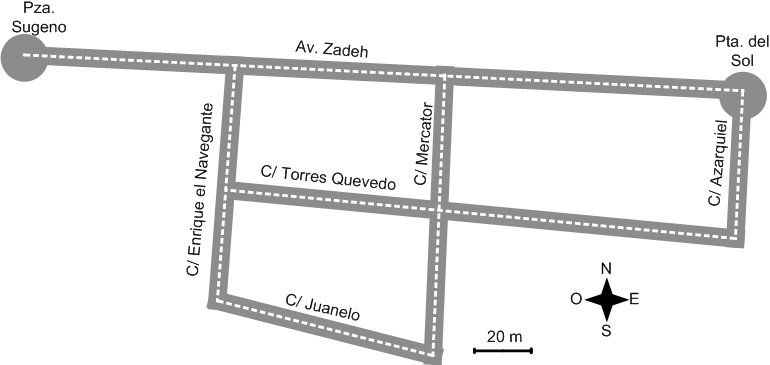
\includegraphics[width=0.5\textwidth]{figures/zocon.png}
  \caption{Plano esquemático de ZOCO}
  \label{fig:zocon}
\end{figure}